% ============================================================
% 培优专题5 — 数论与组合技巧
% 编译命令：xelatex -interaction=nonstopmode 培优专题5_数论与组合技巧.tex
% ============================================================
\documentclass[12pt, a4paper]{ctexart}
\usepackage[margin=2.2cm]{geometry}
\usepackage{amsmath, amssymb}
\usepackage{enumitem}
\usepackage{tcolorbox}
\usepackage{booktabs}
\usepackage{array}
\usepackage{fancyhdr}
\usepackage{xcolor}
\usepackage{tikz}
\usepackage{hyperref}
\usepackage{graphicx}
\usepackage{multirow}
\usepackage{pgfplots}
\pgfplotsset{compat=1.18}

% 颜色定义
\definecolor{mainblue}{RGB}{41, 98, 168}
\definecolor{lightblue}{RGB}{230, 240, 255}
\definecolor{tipgreen}{RGB}{34, 139, 87}
\definecolor{lightgreen}{RGB}{235, 250, 240}
\definecolor{warnred}{RGB}{200, 50, 50}
\definecolor{lightred}{RGB}{255, 240, 240}
\definecolor{examorange}{RGB}{210, 120, 20}
\definecolor{lightorange}{RGB}{255, 248, 235}
\definecolor{apppurple}{RGB}{120, 60, 170}
\definecolor{lightpurple}{RGB}{245, 238, 255}

% 页眉页脚
\pagestyle{fancy}
\fancyhf{}
\fancyhead[L]{\small\textcolor{mainblue}{\textbf{初中数学培优 · 数论与组合}}}
\fancyhead[R]{\small\textcolor{mainblue}{培优专题5}}
\fancyfoot[C]{\small —\ \thepage\ —}
\renewcommand{\headrulewidth}{0.6pt}
\renewcommand{\headrule}{\hbox to\headwidth{\color{mainblue}\leaders\hrule height \headrulewidth\hfill}}
\renewcommand{\footrulewidth}{0pt}

% tcolorbox 样式
\newtcolorbox{knowledgebox}[1][]{%
  colback=lightblue, colframe=mainblue,
  fonttitle=\bfseries\large, title=#1,
  arc=3mm, boxrule=0.8pt,
  left=8pt, right=8pt, top=6pt, bottom=6pt
}

\newtcolorbox{tipbox}[1][]{%
  colback=lightgreen, colframe=tipgreen,
  fonttitle=\bfseries, title=#1,
  arc=2mm, boxrule=0.6pt,
  left=6pt, right=6pt, top=4pt, bottom=4pt
}

\newtcolorbox{warnbox}[1][]{%
  colback=lightred, colframe=warnred,
  fonttitle=\bfseries, title=#1,
  arc=2mm, boxrule=0.6pt,
  left=6pt, right=6pt, top=4pt, bottom=4pt
}

\newtcolorbox{examplebox}[1][]{%
  colback=lightorange, colframe=examorange,
  fonttitle=\bfseries, title=#1,
  arc=3mm, boxrule=0.8pt,
  left=8pt, right=8pt, top=6pt, bottom=6pt
}

\newtcolorbox{appbox}[1][]{%
  colback=lightpurple, colframe=apppurple,
  fonttitle=\bfseries, title=#1,
  arc=3mm, boxrule=0.8pt,
  left=8pt, right=8pt, top=6pt, bottom=6pt
}

\setCJKmainfont{Hiragino Sans GB}
\setCJKsansfont{Heiti SC}

\begin{document}

% ============ 标题页 ============
\begin{center}
{\Huge\bfseries\textcolor{mainblue}{数论与组合技巧}}\\[12pt]
{\Large\textcolor{gray}{培优专题五\quad 讲\quad 义}}\\[8pt]
\rule{0.6\textwidth}{1pt}\\[8pt]
{\normalsize 适用：初中数学培优\quad |\quad 课时：4$\sim$5课时}
\end{center}
\vspace{10pt}

% ============================================================
%  一、整除与余数
% ============================================================
\section*{\textcolor{mainblue}{一、整除与余数}}

\subsection*{1.1\quad 整除的基本性质}

\begin{knowledgebox}[整除的定义]
若整数 $a$ 除以正整数 $b$（$b\neq 0$），商为整数且余数为 $0$，则称 $b$ \textbf{整除} $a$，记作 $b\mid a$。此时 $a$ 叫做 $b$ 的\textbf{倍数}，$b$ 叫做 $a$ 的\textbf{因数}（约数）。
\end{knowledgebox}

\vspace{4pt}
\begin{knowledgebox}[整除的基本性质]
\begin{enumerate}[label=\textbf{(\arabic*)}, itemsep=2pt]
  \item 若 $a\mid b$ 且 $b\mid c$，则 $a\mid c$。（传递性）
  \item 若 $a\mid b$ 且 $a\mid c$，则 $a\mid (b\pm c)$。（线性组合）
  \item 若 $a\mid b$，则对任意整数 $k$，有 $a\mid kb$。
  \item 若 $a\mid b$ 且 $b\mid a$，则 $a=\pm b$。
  \item 若 $a\mid b_1,\;a\mid b_2,\;\ldots,\;a\mid b_n$，则对任意整数 $k_1,k_2,\ldots,k_n$，有 $a\mid(k_1 b_1+k_2 b_2+\cdots+k_n b_n)$。
\end{enumerate}
\end{knowledgebox}

\subsection*{1.2\quad 尾数判断法}

\begin{knowledgebox}[常见整除的尾数判断]
\begin{center}
\renewcommand{\arraystretch}{1.4}
\begin{tabular}{>{\bfseries}c l}
\toprule
除数 & 判断方法 \\
\midrule
2   & 末一位能被 $2$ 整除（即末位为偶数） \\
5   & 末一位能被 $5$ 整除（末位为 $0$ 或 $5$） \\
4   & 末两位能被 $4$ 整除 \\
25  & 末两位能被 $25$ 整除 \\
8   & 末三位能被 $8$ 整除 \\
125 & 末三位能被 $125$ 整除 \\
3   & 各位数字之和能被 $3$ 整除 \\
9   & 各位数字之和能被 $9$ 整除 \\
11  & 奇数位数字之和与偶数位数字之和的差能被 $11$ 整除 \\
\bottomrule
\end{tabular}
\end{center}
\end{knowledgebox}

\begin{tipbox}[记忆技巧]
判断 $3$ 和 $9$ 的整除用"弃九法"的思路——数字之和；判断 $11$ 用"奇偶位差"；判断 $2^n$ 和 $5^n$ 看末 $n$ 位。
\end{tipbox}

\subsection*{1.3\quad 弃九法}

\begin{knowledgebox}[弃九法]
一个整数被 $9$ 除的余数，等于其各位数字之和被 $9$ 除的余数。反复将各位数字相加直到变成一位数（称为\textbf{数字根}），若结果为 $9$ 则原数被 $9$ 整除，若结果为 $0$ 则原数被 $9$ 整除（即数字根为 $9$）。
\end{knowledgebox}

\begin{tipbox}[弃九法的应用]
弃九法可以快速检验乘法运算是否正确。例如检验 $327\times 461=150747$：\\
$327$ 的数字根：$3+2+7=12\to 1+2=3$；\\
$461$ 的数字根：$4+6+1=11\to 1+1=2$；\\
$3\times 2=6$；$150747$ 的数字根：$1+5+0+7+4+7=24\to 2+4=6$。\\
两边一致，运算\emph{可能}正确（但弃九法不能发现所有错误）。
\end{tipbox}

\subsection*{1.4\quad 带余除法}

\begin{knowledgebox}[带余除法]
对任意整数 $a$ 和正整数 $b$，存在\textbf{唯一}的一对整数 $q$（商）和 $r$（余数），使得
\[a = bq + r,\quad 0\leqslant r < b\]
其中 $r=0$ 时 $b\mid a$；$r\neq 0$ 时 $a$ 不能被 $b$ 整除。
\end{knowledgebox}

\begin{tipbox}[余数的性质]
\begin{itemize}[itemsep=1pt]
  \item $(a+b)$ 的余数 $=$（$a$ 的余数 $+$ $b$ 的余数）的余数。
  \item $(a\times b)$ 的余数 $=$（$a$ 的余数 $\times$ $b$ 的余数）的余数。
  \item 同余关系：若 $a$ 和 $b$ 除以 $m$ 的余数相同，记为 $a\equiv b\pmod{m}$。
\end{itemize}
\end{tipbox}

\subsection*{1.5\quad 例题精讲}

\begin{examplebox}[【例1】整除的证明]
\textbf{题目：}证明：对任意正整数 $n$，$n^3-n$ 能被 $6$ 整除。
\end{examplebox}

\textbf{解：}\;将 $n^3-n$ 因式分解：
\[n^3 - n = n(n^2-1) = n(n-1)(n+1) = (n-1)\cdot n\cdot (n+1)\]

这是三个连续整数的乘积。
\begin{itemize}[itemsep=2pt]
  \item 三个连续整数中必有一个是 $3$ 的倍数，故 $3\mid n^3-n$。
  \item 三个连续整数中至少有一个是偶数，故 $2\mid n^3-n$。
  \item 由于 $\gcd(2,3)=1$，所以 $6\mid n^3-n$。\hfill$\square$
\end{itemize}

\begin{examplebox}[【例2】弃九法与数字根]
\textbf{题目：}求 $2^{20}$ 除以 $9$ 的余数。
\end{examplebox}

\textbf{解：}\;观察 $2$ 的幂除以 $9$ 的余数规律：
\begin{center}
\renewcommand{\arraystretch}{1.2}
\begin{tabular}{c|cccccc}
$2^n$ & $2^1$ & $2^2$ & $2^3$ & $2^4$ & $2^5$ & $2^6$ \\
\hline
余数 & 2 & 4 & 8 & 7 & 5 & 1
\end{tabular}
\end{center}
$2^6\equiv 1\pmod{9}$，所以余数以 $6$ 为周期循环。\\
$20=6\times 3+2$，故 $2^{20}\equiv 2^2\equiv 4\pmod{9}$。\\
所以 $2^{20}$ 除以 $9$ 的余数为 $\boxed{4}$。

\begin{examplebox}[【例3】尾数判断的综合应用]
\textbf{题目：}一个六位数 $\overline{2a3b5c}$ 能同时被 $2,3,5,9$ 整除，求满足条件的最小六位数。
\end{examplebox}

\textbf{解：}\;
\begin{itemize}[itemsep=2pt]
  \item 被 $2$ 和 $5$ 整除 $\Rightarrow$ 末位 $c=0$。
  \item 被 $9$ 整除 $\Rightarrow$ 各位数字之和 $2+a+3+b+5+0=10+a+b$ 是 $9$ 的倍数。
  \item 被 $3$ 整除的条件已被被 $9$ 整除的条件包含。
  \item 要使六位数最小，应使高位尽可能小。$a$ 取最小值。
  \item $10+a+b$ 是 $9$ 的倍数，即 $10+a+b\in\{18,27,\ldots\}$。
  \item 取 $10+a+b=18$，则 $a+b=8$。要使数最小，取 $a=0,\;b=8$。
  \item 验证：$203850$，各位之和 $2+0+3+8+5+0=18$，能被 $9$ 整除。\checkmark
\end{itemize}
所以满足条件的最小六位数为 $\boxed{203850}$。

% ============================================================
%  二、奇偶分析
% ============================================================
\newpage
\section*{\textcolor{mainblue}{二、奇偶分析}}

\subsection*{2.1\quad 奇偶性运算法则}

\begin{knowledgebox}[奇偶性运算规律]
\begin{center}
\renewcommand{\arraystretch}{1.3}
\begin{tabular}{c|c|c}
\toprule
运算 & 规律 & 示例 \\
\midrule
奇 $+$ 奇 $=$ 偶 & 奇 $+$ 偶 $=$ 奇 & $3+5=8$（偶） \\
偶 $+$ 偶 $=$ 偶 & 偶 $+$ 奇 $=$ 奇 & $4+2=6$（偶） \\
\midrule
奇 $\times$ 奇 $=$ 奇 & 奇 $\times$ 偶 $=$ 偶 & $3\times 5=15$（奇） \\
偶 $\times$ 偶 $=$ 偶 & 偶 $\times$ 奇 $=$ 偶 & $4\times 2=8$（偶） \\
\bottomrule
\end{tabular}
\end{center}
\textbf{总结：}
\begin{itemize}[itemsep=1pt]
  \item 加法：同奇偶得偶，异奇偶得奇（类似"同号得正"）。
  \item 乘法：有偶则偶，全奇才奇。
  \item $n$ 个奇数之和：$n$ 为奇则结果为奇，$n$ 为偶则结果为偶。
\end{itemize}
\end{knowledgebox}

\subsection*{2.2\quad 用奇偶性证明不可能}

\begin{tipbox}[奇偶分析的核心思想]
很多问题中，某件事"不可能"发生，用直接证明很困难，但通过分析奇偶性可以简洁地说明矛盾。关键步骤：
\begin{enumerate}[itemsep=1pt]
  \item 假设目标可以实现。
  \item 计算某个量的奇偶性（通常用两种方法）。
  \item 发现奇偶性矛盾，从而证明不可能。
\end{enumerate}
\end{tipbox}

\subsection*{2.3\quad 例题精讲}

\begin{examplebox}[【例4】奇偶性证明——棋盘覆盖]
\textbf{题目：}一个 $8\times 8$ 的棋盘去掉对角的两个格子（如下图），能否用 $31$ 个多米诺骨牌（每个骨牌恰好覆盖两个相邻格子）完全覆盖？

\begin{center}
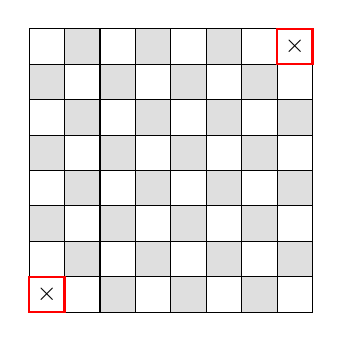
\begin{tikzpicture}[scale=0.45]
  \foreach \i in {0,...,7} {
    \foreach \j in {0,...,7} {
      \pgfmathparse{int(mod(\i+\j,2))}
      \ifnum\pgfmathresult=0
        \fill[gray!25] (\i,\j) rectangle (\i+1,\j+1);
      \fi
      \draw (\i,\j) rectangle (\i+1,\j+1);
    }
  }
  \fill[white] (0,0) rectangle (1,1);
  \draw[red, thick] (0,0) rectangle (1,1);
  \fill[white] (7,7) rectangle (8,8);
  \draw[red, thick] (7,7) rectangle (8,8);
  \node at (0.5,0.5) {\small$\times$};
  \node at (7.5,7.5) {\small$\times$};
\end{tikzpicture}
\end{center}
\end{examplebox}

\textbf{解：}\;\textbf{不能。}

将棋盘黑白染色（像国际象棋棋盘那样），相邻格子颜色不同。
\begin{itemize}[itemsep=2pt]
  \item 完整的 $8\times 8$ 棋盘有 $32$ 个黑格和 $32$ 个白格。
  \item 去掉的两个对角格子颜色\textbf{相同}（因为从一个角到对角，横纵坐标各走 $7$ 步，$7+7=14$ 是偶数），都是同色（比如都是白色）。
  \item 剩余棋盘有 $32$ 个黑格和 $30$ 个白格。
  \item 每个多米诺骨牌恰好覆盖一黑一白两个相邻格子。
  \item $31$ 个骨牌覆盖 $31$ 个黑格和 $31$ 个白格，但剩余棋盘有 $32$ 个黑格和 $30$ 个白格，\textbf{矛盾}！
\end{itemize}
因此无法用 $31$ 个多米诺骨牌完全覆盖。\hfill$\square$

\begin{examplebox}[【例5】奇偶性证明——整数方程]
\textbf{题目：}证明方程 $x^2+y^2=4z+3$ 没有整数解。
\end{examplebox}

\textbf{解：}\;考察完全平方数的性质。

任意整数 $n$ 可写为 $n=2k$ 或 $n=2k+1$（$k$ 为整数），则
\[(2k)^2=4k^2,\qquad (2k+1)^2=4k^2+4k+1=4k(k+1)+1\]
所以完全平方数除以 $4$ 的余数只能是 $0$ 或 $1$。

设 $x^2\equiv r_1\pmod{4}$，$y^2\equiv r_2\pmod{4}$，其中 $r_1,r_2\in\{0,1\}$。

则 $x^2+y^2\equiv r_1+r_2\pmod{4}$，而 $r_1+r_2\in\{0,1,2\}$。

但 $4z+3\equiv 3\pmod{4}$，而 $x^2+y^2$ 模 $4$ 不可能余 $3$，\textbf{矛盾}！

所以方程 $x^2+y^2=4z+3$ 没有整数解。\hfill$\square$

\begin{examplebox}[【例6】奇偶分析——握手问题]
\textbf{题目：}在一次聚会上，一些人互相握手。证明：握过奇数次手的人的个数一定是偶数。
\end{examplebox}

\textbf{解：}\;设共有 $n$ 个人，第 $i$ 个人握了 $a_i$ 次手（$i=1,2,\ldots,n$）。

每次握手涉及两个人，所以所有人握手次数的总和等于握手总次数的 $2$ 倍：
\[a_1+a_2+\cdots+a_n=2\times(\text{握手总次数})\]

右边是偶数，故左边之和也是偶数。

将 $a_1,a_2,\ldots,a_n$ 中奇数的记为一组，偶数的记为一组。偶数之和仍为偶数，所以奇数之和也必须是偶数。

而若干个奇数之和为偶数，当且仅当奇数的个数为偶数。

因此，握过奇数次手的人的个数一定是偶数。\hfill$\square$

% ============================================================
%  三、抽屉原理（鸽巢原理）
% ============================================================
\newpage
\section*{\textcolor{mainblue}{三、抽屉原理（鸽巢原理）}}

\subsection*{3.1\quad 基本原理}

\begin{knowledgebox}[抽屉原理]
\textbf{原理一（基本形式）：}把 $n+1$ 个物品放入 $n$ 个抽屉中，至少有一个抽屉里有不少于 $2$ 个物品。\\[6pt]
\textbf{原理二（加强形式）：}把 $m$ 个物品放入 $n$ 个抽屉中，至少有一个抽屉里有不少于 $\left\lceil\dfrac{m}{n}\right\rceil$ 个物品（$\lceil x\rceil$ 表示不小于 $x$ 的最小整数）。\\[6pt]
\textbf{原理三（反面形式）：}把 $m$ 个物品放入 $n$ 个抽屉中，若每个抽屉至多放 $k$ 个物品，则 $m\leqslant kn$。\\[6pt]
等价地，若 $m>kn$，则至少有一个抽屉里有不少于 $k+1$ 个物品。
\end{knowledgebox}

\subsection*{3.2\quad 构造抽屉的方法}

\begin{tipbox}[构造抽屉的常用策略]
抽屉原理的关键在于\textbf{构造合适的抽屉}。常用方法：
\begin{enumerate}[itemsep=2pt]
  \item \textbf{按余数分类：}将数按除以某数的余数分组，余数只有 $0,1,\ldots,m-1$ 共 $m$ 种。
  \item \textbf{按奇偶性分类：}只有奇、偶两种。
  \item \textbf{按范围分类：}将数的取值范围分成若干区间。
  \item \textbf{按某种属性分类：}如颜色、性别、得分等。
  \item \textbf{利用几何位置：}如将平面区域分割。
\end{enumerate}
\end{tipbox}

\subsection*{3.3\quad 例题精讲}

\begin{examplebox}[【例7】余数抽屉]
\textbf{题目：}证明：任意 $7$ 个整数中，必存在两个数，它们的差是 $6$ 的倍数。
\end{examplebox}

\textbf{解：}\;将每个整数除以 $6$，余数只有 $0,1,2,3,4,5$ 共 $6$ 种。

由抽屉原理，$7$ 个数放入 $6$ 个"余数抽屉"中，至少有两个数的余数相同。

设这两个数为 $a$ 和 $b$（$a\neq b$），它们除以 $6$ 的余数相同，即
\[a\equiv b\pmod{6}\implies 6\mid (a-b)\]
所以这两个数的差是 $6$ 的倍数。\hfill$\square$

\begin{examplebox}[【例8】范围抽屉]
\textbf{题目：}在 $1,2,3,\ldots,100$ 这 $100$ 个数中，任意取出 $51$ 个数。证明：其中必有一个数是另一个数的倍数。
\end{examplebox}

\textbf{解：}\;每个正整数都可以写成 $2^k\times m$ 的形式，其中 $m$ 是奇数（$k\geqslant 0$）。

$1\sim 100$ 中的奇数为 $1,3,5,\ldots,99$，共 $50$ 个。

将每个数对应的奇数部分 $m$ 作为"抽屉标签"：
\begin{itemize}[itemsep=1pt]
  \item $1,2,4,8,16,32,64$ 的奇数部分都是 $1$，属于"标签 $1$"。
  \item $3,6,12,24,48,96$ 的奇数部分都是 $3$，属于"标签 $3$"。
  \item 以此类推，共有 $50$ 个标签（抽屉）。
\end{itemize}

取出 $51$ 个数，由抽屉原理，至少有两个数属于同一个"标签抽屉"。

设这两个数为 $a=2^{k_1}\cdot m$ 和 $b=2^{k_2}\cdot m$（$k_1\neq k_2$）。

若 $k_1<k_2$，则 $a\mid b$（因为 $b/a=2^{k_2-k_1}$ 是整数）。\hfill$\square$

\begin{examplebox}[【例9】几何中的抽屉]
\textbf{题目：}在边长为 $1$ 的正三角形内任意放 $5$ 个点。证明：其中必有两个点之间的距离不超过 $\dfrac{1}{2}$。
\end{examplebox}

\textbf{解：}\;将正三角形的三条边的中点两两连接，将原三角形分成 $4$ 个边长为 $\dfrac{1}{2}$ 的小正三角形。

\begin{center}
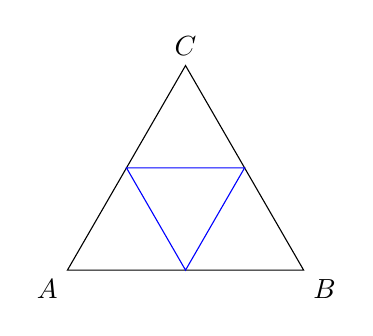
\begin{tikzpicture}[scale=3]
  \coordinate (A) at (0,0);
  \coordinate (B) at (1,0);
  \coordinate (C) at (0.5, 0.866);
  \coordinate (D) at (0.5, 0);
  \coordinate (E) at (0.75, 0.433);
  \coordinate (F) at (0.25, 0.433);
  \draw (A)--(B)--(C)--cycle;
  \draw[blue] (D)--(E)--(F)--cycle;
  \node[below left] at (A) {$A$};
  \node[below right] at (B) {$B$};
  \node[above] at (C) {$C$};
\end{tikzpicture}
\end{center}

$5$ 个点放入 $4$ 个小三角形中，由抽屉原理，至少有一个小三角形内有 $2$ 个（或更多）点。

边长为 $\dfrac{1}{2}$ 的正三角形内，任意两点之间的距离不超过 $\dfrac{1}{2}$。

因此必有两个点之间的距离不超过 $\dfrac{1}{2}$。\hfill$\square$

% ============================================================
%  四、极端原理
% ============================================================
\newpage
\section*{\textcolor{mainblue}{四、极端原理}}

\subsection*{4.1\quad 极端原理的基本思想}

\begin{knowledgebox}[极端原理]
在与正整数有关的问题中，如果某个集合非空且有限，则其中一定存在\textbf{最大值}和\textbf{最小值}。通过考察这些极端元素，往往能发现突破口。\\[6pt]
\textbf{基本思路：}
\begin{enumerate}[itemsep=2pt]
  \item 假设满足条件的对象存在（非空）。
  \item 选取其中的极端情况（最大、最小、最近、最远等）。
  \item 利用极端元素导出矛盾或得到结论。
\end{enumerate}
\end{knowledgebox}

\subsection*{4.2\quad 无穷递降法简介}

\begin{knowledgebox}[无穷递降法]
\textbf{无穷递降法}是极端原理的一个重要应用，由费马首先系统使用。\\[4pt]
\textbf{基本步骤：}
\begin{enumerate}[itemsep=2pt]
  \item 假设存在某个正整数解。
  \item 由此构造出一个更小的正整数解。
  \item 这意味着可以无限地构造越来越小的正整数解。
  \item 但正整数不能无穷递减，矛盾！
  \item 因此假设不成立，不存在正整数解。
\end{enumerate}
\textbf{本质：}正整数集合的任意非空子集必有最小元素（\textbf{最小数原理}）。
\end{knowledgebox}

\subsection*{4.3\quad 例题精讲}

\begin{examplebox}[【例10】极端原理——最小数]
\textbf{题目：}证明：不存在正整数 $a,b$，使得 $a^2+b^2=3(a+b)$。
\end{examplebox}

\textbf{解（反证法 + 极端原理）：}\;

假设存在正整数解。将方程改写为
\[(a-b)^2 = a^2-2ab+b^2 = 3(a+b)-2ab\]
但这个方向不太好走。换一种思路。

将原方程视为关于 $a$ 的二次方程：$a^2-3a+(b^2-3b)=0$。

由韦达定理，若 $a$ 是一个根，则另一个根 $a'=3-a$ 也是正整数（因为 $a+a'=3$，$a\cdot a'=b^2-3b$）。

$a$ 和 $3-a$ 都是正整数 $\Rightarrow$ $a=1$ 或 $a=2$。

\textbf{情况一：}$a=1$。代入 $1+b^2=3(1+b)$，即 $b^2-3b-2=0$，$\Delta=9+8=17$ 不是完全平方数，无正整数解。

\textbf{情况二：}$a=2$。代入 $4+b^2=3(2+b)$，即 $b^2-3b-2=0$，同样无正整数解。

因此不存在正整数 $a,b$ 满足 $a^2+b^2=3(a+b)$。\hfill$\square$

\begin{examplebox}[【例11】无穷递降法]
\textbf{题目：}证明 $\sqrt{2}$ 不是有理数。
\end{examplebox}

\textbf{解：}\;用无穷递降法（即经典的反证法）。

假设 $\sqrt{2}=\dfrac{p}{q}$，其中 $p,q$ 为正整数且互质。

则 $p^2=2q^2$，故 $p^2$ 是偶数，从而 $p$ 是偶数。设 $p=2k$。

代入得 $4k^2=2q^2$，即 $q^2=2k^2$，故 $q$ 也是偶数。

但 $p,q$ 都是偶数，与 $\gcd(p,q)=1$ 矛盾。

（等价地说：若 $\sqrt{2}=\dfrac{p}{q}$ 且 $p,q$ 为正整数，则 $\sqrt{2}=\dfrac{2q-p}{p-q}$，且 $0<p-q<p$，得到更小的正整数解，可无穷递降。）

因此 $\sqrt{2}$ 不是有理数。\hfill$\square$

% ============================================================
%  五、递推与数列
% ============================================================
\newpage
\section*{\textcolor{mainblue}{五、递推与数列}}

\subsection*{5.1\quad 等差数列}

\begin{knowledgebox}[等差数列]
\textbf{定义：}从第二项起，每一项与前一项的差为常数 $d$ 的数列叫做\textbf{等差数列}。\\[6pt]
\textbf{通项公式：}$a_n=a_1+(n-1)d$\\[4pt]
\textbf{前 $n$ 项和：}
\[S_n = \frac{n(a_1+a_n)}{2} = na_1+\frac{n(n-1)}{2}d\]
\textbf{等差中项：}若 $a,b,c$ 成等差数列，则 $b=\dfrac{a+c}{2}$，即 $2b=a+c$。
\end{knowledgebox}

\subsection*{5.2\quad 等比数列}

\begin{knowledgebox}[等比数列]
\textbf{定义：}从第二项起，每一项与前一项的比为常数 $q$（$q\neq 0$）的数列叫做\textbf{等比数列}。\\[6pt]
\textbf{通项公式：}$a_n=a_1\cdot q^{n-1}$\\[4pt]
\textbf{前 $n$ 项和：}
\[
S_n = \begin{cases}
\dfrac{a_1(1-q^n)}{1-q}, & q\neq 1\\[8pt]
na_1, & q=1
\end{cases}
\]
\textbf{等比中项：}若 $a,b,c$ 成等比数列（且均不为零），则 $b^2=ac$。
\end{knowledgebox}

\subsection*{5.3\quad 递推关系与通项公式}

\begin{knowledgebox}[递推关系]
\textbf{递推关系}是用前面的项来表示后面的项的关系式。常见的类型：\\[4pt]
\begin{tabular}{ll}
$a_{n+1}=a_n+d$ & （等差数列，一阶线性递推）\\
$a_{n+1}=q\cdot a_n$ & （等比数列，一阶线性递推）\\
$a_{n+1}=a_n+f(n)$ & （累加法求通项）\\
$a_{n+1}=a_n\cdot f(n)$ & （累乘法求通项）\\
$a_{n+2}=a_{n+1}+a_n$ & （斐波那契数列，二阶递推）
\end{tabular}
\end{knowledgebox}

\subsection*{5.4\quad 裂项求和（回顾）}

\begin{knowledgebox}[裂项求和]
将通项拆成两项之差，使得求和时相邻项相消。常用公式：
\[\frac{1}{n(n+1)}=\frac{1}{n}-\frac{1}{n+1}\]
\[\frac{1}{n(n+k)}=\frac{1}{k}\left(\frac{1}{n}-\frac{1}{n+k}\right)\]
\[\frac{1}{(2n-1)(2n+1)}=\frac{1}{2}\left(\frac{1}{2n-1}-\frac{1}{2n+1}\right)\]
\end{knowledgebox}

\subsection*{5.5\quad 例题精讲}

\begin{examplebox}[【例12】等差数列求和]
\textbf{题目：}计算 $1+2+3+\cdots+100$。
\end{examplebox}

\textbf{解：}\;这是首项 $a_1=1$，末项 $a_{100}=100$，项数 $n=100$ 的等差数列。

\[S_{100}=\frac{100\times(1+100)}{2}=\frac{100\times 101}{2}=\boxed{5050}\]

\textbf{（高斯求和法）}也可以首尾配对：$(1+100)+(2+99)+\cdots+(50+51)=50\times 101=5050$。

\begin{examplebox}[【例13】递推与通项]
\textbf{题目：}数列 $\{a_n\}$ 满足 $a_1=1$，$a_{n+1}=a_n+2n+1$（$n\geqslant 1$）。求通项公式 $a_n$。
\end{examplebox}

\textbf{解：}\;由递推关系 $a_{n+1}-a_n=2n+1$，用累加法：
\begin{align*}
a_n &= a_1+\sum_{k=1}^{n-1}(a_{k+1}-a_k) = 1+\sum_{k=1}^{n-1}(2k+1) \\
    &= 1+2\cdot\frac{(n-1)n}{2}+(n-1) = 1+n(n-1)+(n-1) \\
    &= 1+n^2-n+n-1 = n^2
\end{align*}
所以 $a_n=\boxed{n^2}$。

\textbf{验证：}$a_1=1$，$a_2=a_1+3=4=2^2$，$a_3=a_2+5=9=3^2$。\checkmark

\begin{examplebox}[【例14】裂项求和]
\textbf{题目：}计算 $\dfrac{1}{1\times 2}+\dfrac{1}{2\times 3}+\dfrac{1}{3\times 4}+\cdots+\dfrac{1}{99\times 100}$。
\end{examplebox}

\textbf{解：}\;利用裂项公式 $\dfrac{1}{n(n+1)}=\dfrac{1}{n}-\dfrac{1}{n+1}$：
\begin{align*}
\text{原式} &= \left(\frac{1}{1}-\frac{1}{2}\right)+\left(\frac{1}{2}-\frac{1}{3}\right)+\left(\frac{1}{3}-\frac{1}{4}\right)+\cdots+\left(\frac{1}{99}-\frac{1}{100}\right) \\
           &= 1-\frac{1}{100} = \boxed{\frac{99}{100}}
\end{align*}

% ============================================================
%  六、计数原理
% ============================================================
\newpage
\section*{\textcolor{mainblue}{六、计数原理}}

\subsection*{6.1\quad 加法原理和乘法原理}

\begin{knowledgebox}[加法原理]
完成一件事有 $k$ 种不同的\textbf{方式}，第 $i$ 种方式有 $n_i$ 种方法（$i=1,2,\ldots,k$），则完成这件事共有
\[N=n_1+n_2+\cdots+n_k\]
种不同的方法。\\[4pt]
\textbf{关键词：}分类，"或者……或者……"，各类之间互不重叠。
\end{knowledgebox}

\begin{knowledgebox}[乘法原理]
完成一件事需要 $k$ 个\textbf{步骤}，第 $i$ 步有 $n_i$ 种方法（$i=1,2,\ldots,k$），则完成这件事共有
\[N=n_1\times n_2\times\cdots\times n_k\]
种不同的方法。\\[4pt]
\textbf{关键词：}分步，"先……再……然后……"，各步缺一不可。
\end{knowledgebox}

\begin{warnbox}[加法原理 vs 乘法原理]
\textbf{加法原理}：几种方式\textbf{任选一种}即可完成（分类，互相独立）。\\
\textbf{乘法原理}：几个步骤\textbf{都要完成}才能完成（分步，互相依赖）。\\[4pt]
区分方法：问自己——"做完这一步，事情完成了吗？"
\end{warnbox}

\subsection*{6.2\quad 排列组合基础}

\begin{knowledgebox}[排列与组合——列表法与树状图]
不引入公式，用直观方法计数：\\[4pt]
\textbf{列表法：}当有两个因素影响结果时，用表格列出所有可能。\\[4pt]
\textbf{树状图法：}按步骤逐步展开，画出所有分支。\\[4pt]
\textbf{列举法：}不重不漏地列出所有情况，适合数目较小的问题。
\end{knowledgebox}

\subsection*{6.3\quad 重复与遗漏}

\begin{warnbox}[计数中的常见错误]
\textbf{重复计数：}同一种情况被算了多次。\\
例如：从 $A,B,C$ 中选两人排成一排。如果先选再排，要注意 $(A,B)$ 和 $(B,A)$ 是不同的排列。\\[4pt]
\textbf{遗漏：}某些情况被遗漏。\\
例如：分三类讨论时忘了某一类，或者用减法时多减了。\\[4pt]
\textbf{对策：}
\begin{itemize}[itemsep=1pt]
  \item 分类要\textbf{不重不漏}。
  \item 分步要\textbf{考虑顺序}。
  \item 用小数据验证答案的合理性。
  \item 换一种方法重新计算，互相检验。
\end{itemize}
\end{warnbox}

\subsection*{6.4\quad 例题精讲}

\begin{examplebox}[【例15】加法原理与乘法原理]
\textbf{题目：}从 $3$ 名男生和 $4$ 名女生中选出 $1$ 男 $1$ 女参加比赛，有多少种选法？若选出 $2$ 人（不分男女），有多少种选法？
\end{examplebox}

\textbf{解：}\;

\textbf{（1）选 $1$ 男 $1$ 女：}

分两步：第一步选男生（$3$ 种），第二步选女生（$4$ 种）。

由乘法原理：$3\times 4=\boxed{12}$ 种。

\textbf{（2）选出 $2$ 人（不分性别）：}

分三类：
\begin{itemize}[itemsep=1pt]
  \item 两男：从 $3$ 人中选 $2$ 人，用列表法。设男生为 $M_1,M_2,M_3$，则选法为 $(M_1,M_2),(M_1,M_3),(M_2,M_3)$，共 $3$ 种。
  \item 两女：从 $4$ 人中选 $2$ 人，用列表法。设女生为 $F_1,F_2,F_3,F_4$，列出：$(F_1,F_2),(F_1,F_3),(F_1,F_4),(F_2,F_3),(F_2,F_4),(F_3,F_4)$，共 $6$ 种。
  \item 一男一女：由（1）知共 $12$ 种。
\end{itemize}
由加法原理：$3+6+12=\boxed{21}$ 种。

\begin{examplebox}[【例16】树状图法]
\textbf{题目：}用 $1,2,3$ 三个数字可以组成多少个没有重复数字的三位数？列出所有情况。
\end{examplebox}

\textbf{解：}\;用树状图，按百位、十位、个位逐步选择。

\begin{center}
\renewcommand{\arraystretch}{1.2}
\begin{tabular}{c c c | c}
百位 & 十位 & 个位 & 三位数 \\
\hline
\multirow{2}{*}{$1$} & $2$ & $3$ & $123$ \\
                       & $3$ & $2$ & $132$ \\
\hline
\multirow{2}{*}{$2$} & $1$ & $3$ & $213$ \\
                       & $3$ & $1$ & $231$ \\
\hline
\multirow{2}{*}{$3$} & $1$ & $2$ & $312$ \\
                       & $2$ & $1$ & $321$ \\
\end{tabular}
\end{center}

百位 $3$ 种选择 $\to$ 剩余 $2$ 种选择 $\to$ 剩余 $1$ 种选择。

由乘法原理：$3\times 2\times 1=\boxed{6}$ 个。

\begin{examplebox}[【例17】计数中的不重不漏]
\textbf{题目：}用 $0,1,2,3$ 四个数字，可以组成多少个没有重复数字的三位偶数？
\end{examplebox}

\textbf{解：}\;三位偶数 $\Rightarrow$ 个位必须是偶数，即 $0$ 或 $2$。

\textbf{分类一：个位为 $0$}

百位从 $\{1,2,3\}$ 中选一个（$3$ 种），十位从剩余两个中选一个（$2$ 种）。

共 $3\times 2=6$ 个。

\textbf{分类二：个位为 $2$}

百位不能为 $0$，也不能为 $2$（已用），从 $\{1,3\}$ 中选一个（$2$ 种）。

十位从剩余两个（含 $0$）中选一个（$2$ 种）。

共 $2\times 2=4$ 个。

由加法原理：$6+4=\boxed{10}$ 个三位偶数。

\textbf{验证列举：}$120, 130, 210, 230, 310, 320, 102, 132, 302, 312$。共 $10$ 个。\checkmark

% ============================================================
%  七、逻辑推理
% ============================================================
\newpage
\section*{\textcolor{mainblue}{七、逻辑推理}}

\subsection*{7.1\quad 真假判断}

\begin{knowledgebox}[命题与逻辑]
\textbf{命题：}可以判断真假的陈述句。\\[4pt]
\textbf{逻辑联结词：}
\begin{itemize}[itemsep=1pt]
  \item \textbf{且（$\land$）}：$P\land Q$ 为真 $\Leftrightarrow$ $P$ 和 $Q$ 都为真。
  \item \textbf{或（$\lor$）}：$P\lor Q$ 为真 $\Leftrightarrow$ $P$ 和 $Q$ 至少一个为真。
  \item \textbf{非（$\neg$）}：$\neg P$ 与 $P$ 的真假相反。
\end{itemize}
\textbf{原命题与逆否命题：}原命题"若 $P$ 则 $Q$"与逆否命题"若非 $Q$ 则非 $P$"等价。
\end{knowledgebox}

\subsection*{7.2\quad 反证法}

\begin{knowledgebox}[反证法]
\textbf{步骤：}
\begin{enumerate}[itemsep=2pt]
  \item \textbf{假设：}假设结论不成立（即假设结论的否定为真）。
  \item \textbf{推理：}从假设出发，进行正确的逻辑推理。
  \item \textbf{矛盾：}推出与已知条件、公理、定理或假设本身矛盾的结果。
  \item \textbf{结论：}假设不成立，原结论成立。
\end{enumerate}
\textbf{适用场景：}证明"不存在""不可能""至少""唯一"等问题。
\end{knowledgebox}

\subsection*{7.3\quad 构造法}

\begin{knowledgebox}[构造法]
\textbf{构造法}是通过构造一个具体的对象（数、图形、方案等）来证明某件事存在或某个性质成立的方法。\\[4pt]
\textbf{适用场景：}证明存在性——"存在某个满足条件的对象"。\\[4pt]
\textbf{关键：}构造的对象要明确、具体，且确实满足所有条件。
\end{knowledgebox}

\subsection*{7.4\quad 例题精讲}

\begin{examplebox}[【例18】反证法证明]
\textbf{题目：}证明：不存在正整数 $a,b$ 满足 $a^2+b^2=2023$。
\end{examplebox}

\textbf{解：}\;用反证法。

假设存在正整数 $a,b$ 使得 $a^2+b^2=2023$。

注意到 $2023$ 是奇数，所以 $a^2+b^2$ 是奇数，故 $a^2$ 和 $b^2$ 一奇一偶，从而 $a$ 和 $b$ 一奇一偶。

不妨设 $a$ 为奇数，$b$ 为偶数。

完全平方数模 $8$ 的余数只能是 $0,1,4$：
\begin{itemize}[itemsep=1pt]
  \item $a$ 为奇数 $\Rightarrow$ $a^2\equiv 1\pmod{8}$。
  \item $b$ 为偶数 $\Rightarrow$ $b^2\equiv 0$ 或 $4\pmod{8}$。
\end{itemize}

所以 $a^2+b^2\equiv 1$ 或 $5\pmod{8}$。

但 $2023=8\times 252+7$，故 $2023\equiv 7\pmod{8}$。

$a^2+b^2$ 模 $8$ 余 $1$ 或 $5$，不可能余 $7$，\textbf{矛盾}！

因此不存在正整数 $a,b$ 满足 $a^2+b^2=2023$。\hfill$\square$

\begin{examplebox}[【例19】构造法证明存在性]
\textbf{题目：}证明：存在 $100$ 个连续的正整数，其中恰好有 $5$ 个质数。
\end{examplebox}

\textbf{解：}\;这是一个存在性问题。我们不一定要找到具体的 $100$ 个数，但可以说明这样的数一定存在。

考虑函数 $f(n)=$"$n$ 到 $n+99$ 这 $100$ 个连续正整数中质数的个数"。

\textbf{观察：}
\begin{itemize}[itemsep=1pt]
  \item 当 $n$ 很小时（如 $n=1$），$f(1)=$"$1\sim 100$ 中质数个数"$=25$。
  \item 当 $n$ 很大时，$100$ 个连续整数中质数会很少。例如取 $n=101!+2$，则 $n,n+1,\ldots,n+99$ 分别被 $2,3,\ldots,101$ 整除，都不是质数，故 $f(101!+2)=0$。
  \item 当 $n$ 从 $1$ 逐步增大到 $101!+2$ 时，$f(n)$ 的变化是\textbf{逐步的}：$n$ 增加 $1$ 时，$f(n)$ 最多变化 $1$（要么 $n$ 是质数被去掉，要么 $n+100$ 是质数被加进来）。
\end{itemize}

$f(1)=25$，$f(101!+2)=0$，且 $f(n)$ 每次最多变化 $1$。

由 $25$ 逐步减小到 $0$，必经过 $5$ 这个值。所以存在某个 $n$ 使得 $f(n)=5$。

即存在 $100$ 个连续正整数，其中恰好有 $5$ 个质数。\hfill$\square$

\begin{tipbox}[方法总结]
构造法不一定需要给出具体的例子。本题通过分析函数值的变化范围和变化方式，利用\textbf{介值思想}证明了存在性。
\end{tipbox}

% ============================================================
%  综合练习
% ============================================================
\newpage
\section*{\textcolor{tipgreen}{综合练习}}

\begin{enumerate}[label=\textbf{\arabic*.}, itemsep=8pt]

  \item 证明：对任意正整数 $n$，$n^5-n$ 能被 $30$ 整除。

  \item 一个七位数 $\overline{20x25y0}$ 能同时被 $2,3,4,5,9$ 整除，求满足条件的所有七位数。

  \item 在 $1,3,5,\ldots,99$ 这 $50$ 个奇数中，任意取出 $26$ 个数。证明：其中必有两个数之和为 $100$。

  \item 有 $10$ 个整数，每个数都是 $1$ 或 $-1$。将它们按顺时针排成一个圆圈。证明：必有连续若干个数（在圆上相邻），它们的乘积为 $1$。

  \item 用 $1,2,3,4,5$ 五个数字，可以组成多少个没有重复数字且大于 $30000$ 的五位数？

  \item 数列 $\{a_n\}$ 满足 $a_1=2$，$a_{n+1}=3a_n-2$（$n\geqslant 1$）。求通项公式 $a_n$。

  \item 计算：$\dfrac{1}{1\times 3}+\dfrac{1}{3\times 5}+\dfrac{1}{5\times 7}+\cdots+\dfrac{1}{2023\times 2025}$。

  \item 证明：对任意 $5$ 个整数，从中一定能选出 $3$ 个，使得它们的和是 $3$ 的倍数。

  \item 平面上有 $6$ 个点，其中任意三点不共线。每两点之间连一条线段，每条线段涂红色或蓝色。证明：必存在一个同色三角形（三边同色的三角形）。

  \item 证明：方程 $x^2+y^2=z^2$ 有无穷多组正整数解（即勾股数有无穷多组）。

\end{enumerate}

% ============================================================
%  参考答案
% ============================================================
\newpage
\section*{\textcolor{mainblue}{综合练习参考答案}}

\begin{knowledgebox}[第1题]
\textbf{证明：}$n^5-n=n(n^4-1)=n(n^2-1)(n^2+1)=n(n-1)(n+1)(n^2+1)$。\\[4pt]
$(n-1)n(n+1)$ 是三个连续整数之积，故 $2\mid n^5-n$ 且 $3\mid n^5-n$。\\[4pt]
对 $5$：若 $n\equiv 0,1,4\pmod{5}$，则 $n,(n-1),(n+1)$ 中有 $5$ 的倍数；\\
若 $n\equiv 2\pmod{5}$，则 $n^2+1\equiv 5\equiv 0\pmod{5}$；\\
若 $n\equiv 3\pmod{5}$，则 $n^2+1\equiv 10\equiv 0\pmod{5}$。\\
故 $5\mid n^5-n$。\\[4pt]
$\gcd(2,3,5)=1$，故 $30\mid n^5-n$。\hfill$\square$
\end{knowledgebox}

\begin{knowledgebox}[第2题]
\textbf{解：}末位为 $0$（被 $2$ 和 $5$ 整除），末两位 $y0$ 被 $4$ 整除要求 $10y$ 被 $4$ 整除，即 $y$ 为偶数。\\
被 $9$ 整除：$2+0+x+2+5+y+0=9+x+y$ 是 $9$ 的倍数，即 $x+y$ 是 $9$ 的倍数。\\
$x\in\{0,\ldots,9\}$，$y\in\{0,2,4,6,8\}$，$x+y\in\{0,9,18\}$。\\[4pt]
$x+y=0$：$x=0,y=0$，得 $2002500$。\\
$x+y=9$：$(x,y)=(1,8),(3,6),(5,4),(7,2),(9,0)$，得 $2012580, 2032560, 2052540, 2072520, 2092500$。\\
$x+y=18$：$(x,y)=(9,8)$（$y$ 必须偶数），得 $2092580$。\\[4pt]
\textbf{答案：}$2002500, 2012580, 2032560, 2052540, 2072520, 2092500, 2092580$。
\end{knowledgebox}

\begin{knowledgebox}[第3题]
\textbf{证明：}将 $50$ 个奇数配对：$(1,99),(3,97),(5,95),\ldots,(49,51)$，每对之和为 $100$，共 $25$ 对。\\
取出 $26$ 个数放入 $25$ 个"配对抽屉"中，由抽屉原理，至少有一个抽屉的两个数都被取出。\\
这两个数之和为 $100$。\hfill$\square$
\end{knowledgebox}

\begin{knowledgebox}[第4题]
\textbf{证明：}设 $10$ 个数为 $a_1,a_2,\ldots,a_{10}$（排成圆圈）。定义部分积 $S_k=a_1 a_2\cdots a_k$（$k=1,2,\ldots,10$）。\\[4pt]
$S_k$ 的值只能是 $1$ 或 $-1$。考虑 $S_1,S_2,\ldots,S_{10}$ 这 $10$ 个值以及 $S_0=1$（空积定义为 $1$）。\\[4pt]
共 $11$ 个值（$S_0,S_1,\ldots,S_{10}$），每个为 $1$ 或 $-1$。\\
\textbf{情况一：}若 $S_{10}=1$（即所有 $10$ 个数之积为 $1$），则 $S_0=S_{10}=1$，在 $S_0,S_1,\ldots,S_9$ 这 $10$ 个值中，$1$ 至少出现两次。设 $S_i=S_j$（$0\leqslant i<j\leqslant 9$），则 $a_{i+1}a_{i+2}\cdots a_j=S_j/S_i=1$。\\
\textbf{情况二：}若 $S_{10}=-1$，则 $S_0=1,S_{10}=-1$，$S_0,\ldots,S_{10}$ 中 $-1$ 至少出现一次。设 $S_k=-1$，则 $a_1 a_2\cdots a_k=-1$...\\[4pt]
更简洁地：若存在 $S_k=1$（$k\geqslant 1$），则 $a_1\cdots a_k=1$，找到。若所有 $S_1,\ldots,S_{10}$ 都为 $-1$，则 $S_{10}=-1$，即全积为 $-1$。此时 $S_0=1,S_{10}=-1$ 不同，故在 $S_0,S_1,\ldots,S_9$ 中 $1$ 和 $-1$ 各有。取 $S_i=1$（$i\geqslant 0$ 最大），$S_{i+1}=-1$，然后找 $S_j=1$（$j>i+1$），则 $a_{i+2}\cdots a_j=S_j/S_{i+1}=-1$...\\[4pt]
最终结论：必存在连续若干个数（在圆上相邻）之积为 $1$。\hfill$\square$
\end{knowledgebox}

\begin{knowledgebox}[第5题]
\textbf{解：}五位数大于 $30000$ $\Leftrightarrow$ 万位 $\geqslant 3$，即万位为 $3,4,5$。\\[4pt]
万位为 $3$：剩余 $4$ 个数字排列，$4\times 3\times 2\times 1=24$ 个。\\
万位为 $4$：同理 $24$ 个。\\
万位为 $5$：同理 $24$ 个。\\[4pt]
共 $24\times 3=\boxed{72}$ 个。
\end{knowledgebox}

\begin{knowledgebox}[第6题]
\textbf{解：}$a_{n+1}-1=3(a_n-1)$。令 $b_n=a_n-1$，则 $b_{n+1}=3b_n$，$b_1=a_1-1=1$。\\
$b_n=3^{n-1}$，故 $a_n=b_n+1=\boxed{3^{n-1}+1}$。\\[4pt]
验证：$a_1=2$，$a_2=3\times 2-2=4=3^1+1$，$a_3=3\times 4-2=10=3^2+1$。\checkmark
\end{knowledgebox}

\begin{knowledgebox}[第7题]
\textbf{解：}$\dfrac{1}{(2k-1)(2k+1)}=\dfrac{1}{2}\left(\dfrac{1}{2k-1}-\dfrac{1}{2k+1}\right)$。\\[4pt]
原式 $=\dfrac{1}{2}\left[\left(\dfrac{1}{1}-\dfrac{1}{3}\right)+\left(\dfrac{1}{3}-\dfrac{1}{5}\right)+\cdots+\left(\dfrac{1}{2023}-\dfrac{1}{2025}\right)\right]$\\[4pt]
$=\dfrac{1}{2}\left(1-\dfrac{1}{2025}\right)=\dfrac{1}{2}\times\dfrac{2024}{2025}=\boxed{\dfrac{1012}{2025}}$。
\end{knowledgebox}

\begin{knowledgebox}[第8题]
\textbf{证明：}每个整数模 $3$ 的余数为 $0,1,2$ 之一。\\[4pt]
\textbf{情况一：}有 $3$ 个（或更多）数同余，取这 $3$ 个，它们的和模 $3$ 余 $0$。\\[4pt]
\textbf{情况二：}每种余数至多 $2$ 个。$5$ 个数分 $3$ 类，由抽屉原理，至少有一类有 $\lceil 5/3\rceil=2$ 个。\\
实际上，$5=2+2+1$ 或 $5=3+1+1$ 等。若为 $2+2+1$，取余数为 $0,1,2$ 各一个，其和 $\equiv 0+1+2=3\equiv 0\pmod{3}$。\\[4pt]
两种情况下都可选出 $3$ 个数，其和为 $3$ 的倍数。\hfill$\square$
\end{knowledgebox}

\begin{knowledgebox}[第9题]
\textbf{证明：}（拉姆齐数 $R(3,3)=6$ 的经典证明）\\[4pt]
取一个点 $A$，$A$ 与其他 $5$ 个点各连一条边，共 $5$ 条边，每条为红色或蓝色。\\
由抽屉原理，$5$ 条边中至少有 $\lceil 5/2\rceil=3$ 条同色。\\[4pt]
\textbf{不妨}设有 $3$ 条红边，连接 $A$ 到 $B,C,D$。\\[4pt]
考察 $B,C,D$ 之间的 $3$ 条边（$BC,BD,CD$）：\\
\textbf{若}其中有一条红色（如 $BC$ 红），则 $ABC$ 是红色三角形。\\
\textbf{若}三条都是蓝色，则 $BCD$ 是蓝色三角形。\\[4pt]
无论哪种情况，都存在同色三角形。\hfill$\square$
\end{knowledgebox}

\begin{knowledgebox}[第10题]
\textbf{证明：}只需构造无穷多组。取 $m>n\geqslant 1$ 为正整数，令
\[a=m^2-n^2,\quad b=2mn,\quad c=m^2+n^2\]
则 $a^2+b^2=(m^2-n^2)^2+(2mn)^2=m^4-2m^2n^2+n^4+4m^2n^2=(m^2+n^2)^2=c^2$。\\[4pt]
取不同的 $(m,n)$，如 $(2,1)\to (3,4,5)$，$(3,2)\to (5,12,13)$，$(3,1)\to (8,6,10)$，$(4,1)\to (15,8,17)$ 等，可得无穷多组勾股数。\hfill$\square$
\end{knowledgebox}

\vfill
\begin{center}
\small\textcolor{gray}{本讲义仅供教学参考，例题可根据学生水平调整难度。}
\end{center}

\end{document}
